\documentclass[a4paper, 12pt, final, garamond]{book}
\usepackage{cours-preambule}

\makeatletter
\renewcommand{\@chapapp}{Architecture de la mati\`ere -- chapitres}
\renewcommand\thechapter{1 et 2}
\makeatother

% \toggletrue{student}
% \HideSolutionstrue
% \toggletrue{corrige}
\renewcommand{\mycol}{black}
% \renewcommand{\mycol}{gray}

\ifx\conditionmacro\undefined
  \immediate\write18{%
    pdflatex --jobname="\currfilebase_enon"
    "\gdef\string\conditionmacro{1}\string\input\space\jobname"
  }%
  \immediate\write18{%
    pdflatex --jobname="\currfilebase_solu-prof"
    "\gdef\string\conditionmacro{2}\string\input\space\jobname"
  }%
  \immediate\write18{%
    pdflatex --jobname="\currfilebase_solu-stud"
    "\gdef\string\conditionmacro{3}\string\input\space\jobname"
  }%
  \expandafter\stop
\fi

\begin{document}
% \setcounter{chapter}{4}

\ifnum\conditionmacro=1 \togglefalse{corrige}\fi
\ifnum\conditionmacro=2 \toggletrue{corrige}\togglefalse{student}\fi
\ifnum\conditionmacro=3 \toggletrue{corrige}\toggletrue{student}\fi

\chapter{\cswitch{Correction du TD}{TD~: structures chimiques et propri\'et\'es
	  macro}}

\resetQ
\section{Structures de \textsc{Lewis}}
\QR{%
	Donner le schéma de \textsc{Lewis} des espèces suivantes~:
	\[
		\ce{CH2Cl2}
		\qquad
		\ce{O2}
		\qquad
		\ce{C2H4}
		\qquad
		\ce{H3O+}
		\qquad
		\ce{HO-}
		\qquad
		\ce{H2CO}
		\qquad
		\ce{SiO2}
		\qquad
		\ce{CH3NH2}
	\]
}{%
	\ifprof{
		\vspace{-20pt}
	}
	\begin{itemize}[label=$\diamond$, leftmargin=10pt]
		\bitem{Dichlorométhane \ce{CH2Cl2}}~:
		\begin{itemize}[label=$\triangleright$, leftmargin=20pt]
			\item Décompte des électrons~:
			      \begin{itemize}[label=$\ra$, leftmargin=20pt]
				      \item $[\ce{H}]~:$ 1 électron de valence
				      \item $[\ce{C}]~:$ 2\ieme\ colonne bloc p,
				            donc 4 électrons de valence
				      \item $[\ce{Cl}]~:$ halogène, 17\ieme\ colonne
				            donc 7 électrons de valence.
				      \item Total~: $2*1 + 4 + 2*7 = 20$ électrons, 10
				            doublets.
			      \end{itemize}
			\item Méthode simple~:
			      \[
				      \cfig{\clew
					      (!{&0}\hlew{4})
					      (!{&2}\hlew{6})
					      (!{&4}\cllew{0})
					      (!{&6}\cllew{2})
				      }
				      \qqdonc
				      \cfig{C(-[0]H)(-[2]H)(-[4]\lewis{246,Cl})(-[6]\lewis{046,Cl})}
			      \]
		\end{itemize}
		\bitem{Dioxygène \ce{O2}}~:
		\begin{itemize}[label=$\triangleright$, leftmargin=20pt]
			\item Décompte des électrons~:
			      \begin{itemize}[label=$\ra$, leftmargin=20pt]
				      \item $[\ce{O}]~:$ 4\ieme\ colonne du bloc p,
				            donc 6 électrons de valence
				      \item Total~: $2*6 = 12$ électrons, 6
				            doublets.
			      \end{itemize}
			\item Méthode simple~:
			      \[
				      \cfig{%
				      \odlew{0}!{&0}\odlew{4}
				      }
				      \qqdonc
				      \cfig{\lewis{35,O}=\lewis{17,O}}
			      \]
		\end{itemize}
		\bitem{Éthène \ce{C2H4}}~:
		\begin{itemize}[label=$\triangleright$, leftmargin=20pt]
			\item Décompte des électrons~:
			      \begin{itemize}[label=$\ra$, leftmargin=20pt]
				      \item $[\ce{H}]~:$ 1 électron de valence
				      \item $[\ce{C}]~:$ 14\ieme\ colonne
				            donc 4 électrons de valence
				      \item Total~: $4*1 + 2*4 = 12$ électrons, 6
				            doublets.
			      \end{itemize}
			\item Méthode simple~:
			      \[
				      \cfig{
					      \lewis{0:2.6.,C}
					      (
					      !{&0}\lewis{2.4:6.,C}
					      (!{&2}\hlew{6})
					      (!{&6}\hlew{2})
					      )
					      (!{&2}\hlew{6})
					      (!{&6}\hlew{2})
				      }
				      \qqdonc
				      \cfig{
				      C(-[2]H)(-[6]H)=C(-[2]H)(-[6]H)
				      }
			      \]
		\end{itemize}
		\bitem{Ion oxonium \ce{H3O+}}~:
		\begin{itemize}[label=$\triangleright$, leftmargin=20pt]
			\item Décompte des électrons~:
			      \begin{itemize}[label=$\ra$, leftmargin=20pt]
				      \item $[\ce{H}]~:$ 1 électron de valence
				      \item $[\ce{O}]~:$ 16\ieme\ colonne donc 6 électrons de valence
				      \item Une charge $\oplus$, donc 1 électron en moins
				      \item Total~: $3*1 + 6 - 1 = 8$ électrons, 4
				            doublets.
			      \end{itemize}
			\item Méthode simple~: \ce{H} est moins électronégatif que
			      \ce{O}, mais si la charge $\oplus$ était portée par un
			      \ce{H} il ne pourrait pas se lier~: c'est forcément
			      \ce{O} qui la porte.
			      \[
				      \cfig{
					      \chemabove{\lewis{0.24.6.,O}}{\vspace{10pt}\hspace{20pt}\oplus}
					      (!{&0}\hlew{4})
					      (!{&4}\hlew{0})
					      (!{&6}\hlew{2})
				      }
				      \qqdonc
				      \cfig{
					      \chemabove{\lewis{2,O}}{\vspace{10pt}\hspace{20pt}\oplus}
					      (-[0]H)
					      (-[4]H)
					      (-[6]H)
				      }
			      \]
		\end{itemize}
		\bitem{Ion hydroxyde \ce{HO-}}~:
		\begin{itemize}[label=$\triangleright$, leftmargin=20pt]
			\item Décompte des électrons~:
			      \begin{itemize}[label=$\ra$, leftmargin=20pt]
				      \item $[\ce{H}]$
				            donc 1 électron de valence
				      \item $[\ce{O}]$ 4\ieme\ colonne bloc p
				            donc 6 électrons de valence
				      \item Une charge $\ominus$, donc 1 électron en plus
				      \item Total~: $1 + 6 + 1 = 8$ électrons, 4
				            doublets.
			      \end{itemize}
			\item Méthode simple~:
			      \[
				      \cfig{\hlew{0}!{&0}\chemabove{\lewis{024.6,O}}{\vspace{10pt}\hspace{20pt}\ominus}}
				      \qdonc
				      \cfig{H-\chemabove{\lewis{026,O}}{\vspace{10pt}\hspace{20pt}\ominus}}
			      \]
		\end{itemize}
		\bitem{Méthanal \ce{H2CO}}~:
		\begin{itemize}[label=$\triangleright$, leftmargin=20pt]
			\item Décompte des électrons~:
			      \begin{itemize}[label=$\ra$, leftmargin=20pt]
				      \item $[\ce{H}]$ 1 électron de valence
				      \item $[\ce{C}]$ 2\ieme\ colonne du bloc p
				            donc 4 électrons de valence
				      \item $[\ce{O}]$ 4\ieme\ colonne du bloc p
				            donc 6 électrons de valence
				      \item Total~: $2*1 + 4 + 6 = 12$ électrons, 6
				            doublets.
			      \end{itemize}
			\item Méthode simple~: on a forcément une liaison \ce{C-O},
			      mais il n'est pas évident de savoir où les \ce{H} vont
			      se lier. On commence donc par les placer entre \ce{C} et
			      \ce{O}.
			      \[
				      \cfig{\vphantom{X}
					      (-[0,0.5,,,draw=none]\odlew{4})
					      (!{&2}\hlew{6})
					      (-[4,0.5,,,draw=none]\lewis{0:2.6.,C})
					      (!{&6}\hlew{2})
				      }
				      \qqdonc
				      \cfig{
				      C
				      (=\lewis{17,O})
				      (-[2]H)
				      (-[6]H)
				      }
			      \]
		\end{itemize}
		\bitem{Dioxyde de silicium \ce{SiO2}}~:
		\begin{itemize}[label=$\triangleright$, leftmargin=20pt]
			\item Décompte des électrons~:
			      \begin{itemize}[label=$\ra$, leftmargin=20pt]
				      \item $[\ce{O}]$ 4\ieme\ colonne du bloc p
				            donc 6 électrons de valence
				      \item $[\ce{Si}]$ famille du carbone
				            donc 4 électrons de valence
				      \item Total~: $2*6 + 4 = 16$ électrons, 8
				            doublets.
			      \end{itemize}
			\item Méthode simple~:
			      \[
				      \cfig{
					      \lewis{0:4:,Si}
					      (!{&0}\odlew{4})
					      (!{&4}\odlew{0})
				      }
				      \qqdonc
				      \cfig{
				      Si
				      (=[0]\lewis{17,O})
				      (=[4]\lewis{35,O})
				      }
			      \]
		\end{itemize}
		\bitem{Méthylamine \ce{CH3NH2}}~:
		\begin{itemize}[label=$\triangleright$, leftmargin=20pt]
			\item Décompte des électrons~:
			      \begin{itemize}[label=$\ra$, leftmargin=20pt]
				      \item $[\ce{H}]$ 1 électron de valence
				      \item $[\ce{C}]$ 2\ieme\ colonne du bloc p
				            donc 4 électrons de valence
				      \item $[\ce{N}]$ 3\ieme\ colonne du bloc p donc
				            5 électrons de valence
				      \item Total~: $5*1 + 4 + 5 = 14$ électrons, 7
				            doublets.
			      \end{itemize}
			\item Méthode simple~: \ce{H} ne peut former qu'une seule
			      liaison, on a forcément une liaison \ce{C-N}.
			      \[
				      \cfig{
					      \clew
					      (!{&0}\hlew{4})
					      (!{&2}\hlew{6})
					      (!{&6}\hlew{2})
					      (!{&4}\nlew{4}
					      (!{&2}\hlew{6})
					      (!{&6}\hlew{2})
					      )
				      }
				      \qqdonc
				      \cfig{
				      C
				      (-[0]H)
				      (-[2]H)
				      (-[6]H)
				      (-[4]\lewis{4,N}
				      (-[2]H)
				      (-[6]H)
				      )
				      }
			      \]
		\end{itemize}
	\end{itemize}
}

\QR{%
	L'ozone \ce{O3} est une molécule non cyclique. Proposer une structure.
}{%
	\ifprof{
		\vspace{-20pt}
	}
	\begin{itemize}
		\bitem{Ozone \ce{O3}}~:
		\begin{itemize}[label=$\triangleright$, leftmargin=20pt]
			\item Décompte des électrons~:
			      \begin{itemize}[label=$\ra$, leftmargin=20pt]
				      \item $[\ce{O}]$ 4\ieme\ colonne du bloc p
				            donc 6 électrons de valence
				      \item Total~: $3*6 = 18$ électrons, 9
				            doublets.
			      \end{itemize}
			\item Méthode simple~: à tenter, mais pas simple d'obtenir
			      un résultat convaincant.
			\item Méthode générale~:
			      \begin{itemize}[label=$\ra$, leftmargin=20pt]
				      \bitem{Squelette}~: immédiat car la molécule est
				      linéaire.
				      \bitem{Recherche de liaisons multiples}~: le squelette
				      implique au moins 2 liaisons, soit 7 doublets
				      restants à placer. \textbf{Si tous les doublets
					      restant étaient non liants}, pour respecter
				      l'octet il en faudrait 3
				      sur les atomes du bout et 2 sur l'atome du
				      milieu, soit $2*3+2 = 8$~: c'est un de plus que
				      disponible. Il y a donc \textbf{une liaison
					      double}.
				      \item On pose donc les doublets.
				            \bitem{Recherche des charges formelles}~:
				            \begin{itemize}[label=$\bullet$, leftmargin=20pt]
					            \item Atome de gauche~: il a 6 électrons qui
					                  l'entourent, contre 6 dans son état isolé~:
					                  pas de charge.
					            \item Atome central~: il a 5 électrons qui
					                  l'entourent, donc une charge $\oplus$.
					            \item Atome de droite~: il a 7 électrons qui
					                  l'entourent, donc une charge $\ominus$.
				            \end{itemize}
			      \end{itemize}
			\item Conclusion~:
			      \[
				      \cfig{\lewis{35,O}=
					      \chemabove{\lewis{2,O}}{\vspace{10pt}\hspace{20pt}\oplus}
					      -\chemabove{\lewis{026,O}}{\vspace{-12pt}\hspace{20pt}\ominus}
				      }
			      \]
		\end{itemize}
	\end{itemize}

}
\begin{blocQR}{}
	\item
	\QR{%
		Donner le schéma de \textsc{Lewis} de l'acide sulfurique
		\ce{H2SO4}. Dans cette molécule, les quatre atomes d'oxygène sont
		reliés à l'atome de soufre.
	}{%
		\ifprof{
			\vspace{-20pt}
		}
		\begin{itemize}
			\bitem{Acide sulfurique \ce{H2SO4}}~:
			\begin{itemize}[label=$\triangleright$, leftmargin=20pt]
				\item Décompte des électrons~:
				      \begin{itemize}[label=$\ra$, leftmargin=20pt]
					      \item $[\ce{H}]$ 1 électron de valence
					      \item $[\ce{O}]$ 6 électrons de valence
					      \item $[\ce{S}]$ famille de l'oxygène
					            donc 6 électrons de valence
					      \item Total~: $2*1 + 6 + 4*6 = 32$ électrons, 16
					            doublets.
				      \end{itemize}
				\item Méthode simple~: on nous donne l'information que
				      les 4 atomes d'oxygène sont reliés au silicium. On a
				      donc le squelette, et on complète les doublets en
				      trouvant les deux liaisons doubles qui évitent les
				      deux charges $\ominus$ sur les oxygènes. Comme le
				      silicium appartient à la 3ème période, il est
				      possible qu'il soit entouré de plus de 4 doublets
				      (hypervalent).
				      \[
					      \cfig{\lewis{0.2:4.6:,S}
						      (!{&0}\lewis{0.24.6,O}
						      !{&0}\hlew{4})
						      (!{&4}\lewis{0.24.6,O}
						      !{&4}\hlew{0})
						      (!{&2}\odlew{6})
						      (!{&6}\odlew{2})
					      }
					      \qqdonc
					      \cfig{
					      S
					      (-[0]\lewis{26,O}-[0]H)
					      (-[4]\lewis{26,O}-[4]H)
					      (=[2]\lewis{13,O})
					      (=[6]\lewis{57,O})
					      }
				      \]
			\end{itemize}
		\end{itemize}

	}
	\QR{%
		En déduire celles des ions \ce{HSO4-} et \ce{SO4^{2-}}.
	}{%
		\ifprof{
			\vspace{-20pt}
		}
		\begin{itemize}
			\bitem{Ions hydrogénosulfate \ce{H2SO4-} et l'ion sulfate \ce{SO4^{2-}}}~:
			\begin{itemize}[label=$\triangleright$, leftmargin=20pt]
				\item Décompte des électrons~:
				      Déjà effectué
				\item Méthode simple~: on enlève un atome d'hydrogène à
				      chaque fois, laissant donc le doublet de la liaison
				      \ce{O-H} sur l'atome d'oxygène correspondant, lui
				      laissant une charge $\ominus$.
				      \[
					      \cfig{
					      S
					      (-[0]\chemabove{\lewis{026,O}}{\hspace{20pt}\ominus})
					      (-[4]\lewis{26,O}-[4]H)
					      (=[2]\lewis{13,O})
					      (=[6]\lewis{57,O})
					      }
					      \qqet
					      \cfig{
					      S
					      (-[0]\chemabove{\lewis{026,O}}{\hspace{20pt}\ominus})
					      (-[4]\chemabove{\lewis{246,O}}{\hspace{-20pt}\ominus})
					      (=[2]\lewis{13,O})
					      (=[6]\lewis{57,O})
					      }
				      \]
			\end{itemize}
		\end{itemize}
	}
\end{blocQR}

\QR{%
	Donner le schéma de \textsc{Lewis} des ions hydrogénocarbonate
	\ce{HCO3-} et carbonate \ce{CO3^{2-}}.
}{%
	\ifprof{
		\vspace{-20pt}
	}
	\begin{itemize}
		\bitem{Ion hydrogénocarbonate \ce{HCO3-}}~:
		\begin{itemize}[label=$\triangleright$, leftmargin=20pt]
			\item Décompte des électrons~:
			      \begin{itemize}[label=$\ra$, leftmargin=20pt]
				      \item $[\ce{H}]$ 1 électron de valence
				      \item $[\ce{C}]$ 4 électrons de valence
				      \item $[\ce{O}]$ 6 électrons de valence
				      \item Une charge $\ominus$, donc un électron en plus
				      \item Total~: $1 + 4 + 3*6 +1 = 24$ électrons, 12
				            doublets.
			      \end{itemize}
			\item Méthode simple~: fonctionne… si on part bien~! \ce{O}
			      est le plus électronégatif des atomes de l'ion, on en
			      déduit que c'est un des oxygènes qui la porte.
			\item Méthode générale~:
			      \begin{itemize}[label=$\ra$, leftmargin=20pt]
				      \bitem{Squelette}~: on pourrait partir avec une
				      solution incluant une liaison \ce{O-O} avec le
				      \ce{H} sur \ce{C}, mais comme on sait qu'on va
				      former \ce{CO3^{2-}} ensuite, il faut pouvoir
				      enlever l'atome d'hydrogène sans se retrouver avec
				      \cfig{\charge{30:4pt=$\ominus$,90=\|}{C}}~ qui
				      est très peu commun. On mettra comme d'habitude
				      l'atome qui fait le plus de liaisons au centre, avec
				      l'hydrogène lié à un oxygène.
				      \bitem{Recherche de liaisons multiples}~: le squelette
				      implique au moins 4 liaisons, soit 8 doublets
				      restants à placer. \textbf{Si tous les doublets
					      restant étaient non liants}, pour respecter
				      l'octet il en faudrait 9 en tout~: c'est un de plus que
				      disponible. Il y a donc \textbf{une liaison
					      double}, une \cfig{C=[,.7]O}.
				      \item On pose donc les doublets.
				            \bitem{Recherche des charges formelles}~:
				            \begin{itemize}[label=$\bullet$, leftmargin=20pt]
					            \item Oxygène en haut~: il a 7 électrons qui
					                  l'entourent, contre 6 dans son état isolé~:
					                  charge $\ominus$.
					            \item Carbone~: il a 4 électrons qui
					                  l'entourent, donc pas de charge.
					            \item Autres oxygène~: ils ont 6 électrons qui
					                  les entourent, donc pas de charge.
				            \end{itemize}
			      \end{itemize}
			\item Conclusion~:
			      \[
				      \cfig{
					      \clew
					      (!{&0}\odlew{4})
					      (!{&6}\odlew{2})
					      (!{&4}\hlew{0})
					      (!{&2}\chemabove{\lewis{0246.,O}}{\hspace{20pt}\ominus})
				      }
				      \qqdonc
				      \cfig{
				      C
				      (=[0]\lewis{17,O})
				      (-[2]\chemabove{\lewis{024,O}}{\hspace{20pt}\ominus})
				      (-[6]\lewis{46,O}-[0]H)
				      }
			      \]
		\end{itemize}
		\bitem{Ion carbonate \ce{CO3^{2-}}}~:
		\begin{itemize}[label=$\triangleright$, leftmargin=20pt]
			\item Décompte des électrons~: déjà fait
			\item Méthode simple~: on enlève un hydrogène en rabattant
			      le doublet liant en non-liant.
			      \[
				      \cfig{
				      C
				      (=[0]\lewis{17,O})
				      (-[2]\chemabove{\lewis{024,O}}{\hspace{20pt}\ominus})
				      (-[6]\chemabove{\lewis{046,O}}{\hspace{20pt}\ominus})
				      }
			      \]
		\end{itemize}
	\end{itemize}

}

\QR{%
	Donner le schéma de \textsc{Lewis} du benzène \ce{C6H6}, qui est une
	molécule cyclique.
}{%
	\ifprof{
		\vspace{-20pt}
	}
	\begin{itemize}
		\bitem{Benzène \ce{C6H6}}~:
		\begin{itemize}[label=$\triangleright$, leftmargin=20pt]
			\item Décompte des électrons~:
			      \begin{itemize}[label=$\ra$, leftmargin=20pt]
				      \item $[\ce{H}]$ 1 électron de valence
				      \item $[\ce{C}]$ 4 électrons de valence
				      \item Total~: $6*1 + 6*4 = 30$ électrons, 15
				            doublets.
			      \end{itemize}
			\item Méthode simple~: comme on sait que la molécule est
			      cyclique, il est plus simple de représenter le cycle dès
			      le départ avec des liaisons simples. Ensuite, chaque
			      \ce{H} est lié à un \ce{C}. On a donc consommé $6+6=12$
			      doublets pour ce squelette, il en reste 3 qui ne peuvent
			      être des doublets non liants (sinon charge formelle)~:
			      il a donc 3 liaisons doubles.
			      \[
				      \cfig{
					      \lewis{3.5.,C}
					      (!{&4}\lewis{0.,H})
					      *6
					      (-\lewis{4.6.,C}
					      (!{&5}\lewis{1.,H})
					      -\lewis{0.6.,C}
					      (!{&7}\lewis{3.,H})
					      -\lewis{7.1.,C}
					      (!{&0}\lewis{4.,H})
					      -\lewis{0.2.,C}
					      (!{&1}\lewis{5.,H})
					      -\lewis{2.4.,C}
					      (!{&3}\lewis{7.,H})
					      -
					      )}
				      \qqdonc
				      \cfig{
				      C
				      (-[4]H)
				      *6
				      (=C
				      (-[:-120]H)
				      -C
				      (-[:-60]H)
				      =C
				      (-[0]H)
				      -C
				      (-[:60]H)
				      =C
				      (-[:120]H)
				      -)
				      }
			      \]
		\end{itemize}
	\end{itemize}

}


\resetQ
\section{Le phosphore}
\QR{%
	Donner le nombre d'électrons de valence du phosphore \ce{P}.
}{%
	Famille de l'azote, 3\ieme\ colonne du bloc p, 15\ieme\ colonne du tableau~: 5
	électrons de valence.
}
\QR{%
	Donner la représentation de \textsc{Lewis} de la molécule \ce{PCl3}.
}{%
	Le chlore est un halogène, d'où 7 électrons de valence. On met donc le phosphore
	au centre de l'édifice pour obtenir~:
	\[
		\cfig{
			\lewis{0.2.46.,P}
			(!{&0}\lewis{6024.,Cl})
			(!{&2}\lewis{6.024,Cl})
			(!{&6}\lewis{602.4,Cl})
		}
		\qqdonc
		\cfig{
			\lewis{4,P}
			(-[0]\lewis{026,Cl})
			(-[2]\lewis{024,Cl})
			(-[6]\lewis{046,Cl})
		}
	\]
}

\QR{%
Le phosphore peut aussi former \ce{PCl5}, pourquoi~? Préciser sa
structure de \textsc{Lewis}.
}{%
Le phosphore appartient à la troisième période, et peut donc être
hypervalent (grâce à la sous-couche $d$ non-remplie). On obtient alors
\[
	\cfig{
	P
	(-[0]\lewis{026,Cl})
	(-[2]\lewis{024,Cl})
	(-[3]\lewis{246,Cl})
	(-[5]\lewis{246,Cl})
	(-[6]\lewis{046,Cl})
	}
\]
}

\resetQ
\section{Caractéristiques de quelques solvants}
\enonce{%
	On s'intéresse aux solvants suivants~:
	\begin{table}[ht]
		\centerfloat
		% \caption{Caractéristiques de solvants.}
		\begin{threeparttable}
			\label{tab:solvtd}
			\begin{tabular}{p{3.5cm}ccccc}
				\toprule
				Nom                                                                   &
				Eau                                                                   &
				Méthanol                                                              &
				Hexane                                                                &
				DMF\tnote{1}                                                          &
				Acétonitrile
				\\\midrule
				Représentation                                                        &
				\cfig{\lewis{13,O}(-[5,.7]H)(-[7,.7]H)}                               &
				\cfig{CH_3-[,.7]\lewis{26,O}-[,.7]H}                                  &
				\cfig{CH_3-{{(CH_2)}_4}-CH_3}                                         &
				\cfig{N(-[3,.7]CH_3)(-[5,.7]CH_3)-[,.7]C(=[6,.7]\lewis{57,O})-[,.7]H} &
				\cfig{CH_3-[,.7]C~[,.7]\lewis{0,N}}
				\\[2.3em]\midrule\addlinespace
				Moment dipolaire                                                      &
				\SI{1.8}{D}                                                           &
				\SI{1.65}{D}                                                          &
				\SI{0}{D}                                                             &
				\SI{3.8}{D}                                                           &
				\SI{3.9}{D}
				\\\midrule
				\shortstack[l]{Permittivité                                             \\ relative ($\ep_r$)} &
				\num{78.5}                                                            &
				\num{32.6}                                                            &
				\num{2.0}                                                             &
				\num{36.7}                                                            &
				\num{37.5}
				\\\bottomrule
			\end{tabular}
			\begin{tablenotes}[flushleft]
				\item[1] DMF est l'abréviation de diméthylformamide.
			\end{tablenotes}
		\end{threeparttable}
	\end{table}
}

\QR{%
	Identifier les solvants polaires et apolaires.
}{%
	Tous sont polaires, sauf l'hexane.
}

\QR{%
	Identifier les solvants protiques et aprotiques.
}{%
	L'eau et le méthanol sont protiques, pas les autres.
}

\QR{%
	Identifier les solvants peu dispersifs, dispersifs, fortement
	dispersifs.
}{%
	L'hexane n'est pas dispersif, le méthanol, le DMF et l'acétonitrile
	sont dispersifs, l'eau est fortement dispersive.
}

\QR{%
	Tous ces solvant sont miscibles entre eux, à l'exception de l'hexane.
	Expliquer pourquoi.
}{%
	La présence d'un moment dipolaire sur chacune de ces molécules permet
	des interactions attractives de \textsc{Van der Waals}. L'hexane ne
	présente pas ces propriétés et ne se mélange donc pas bien aux autres.
}

\resetQ
\section{Températures de changements d'état}
\enonce{%
	On indique ci-après les valeurs de température d'ébullition de composés
	apolaires~:
	\begin{table}[ht]
		\centering
		\label{tab:tebapo}
		\begin{tabular}{lcccccc}
			\toprule
			Corps                 &
			\ce{H2}               & \ce{N2}  & \ce{O2}  & \ce{F2}  & \ce{Cl2}  & \ce{Br2}
			\\\midrule
			$T_{\rm eb} (\si{K})$ &
			\num{20}              & \num{77} & \num{90} & \num{85} & \num{238} & \num{331}
			\\\bottomrule
		\end{tabular}
	\end{table}
}

\QR{%
	Interpréter l'évolution constatée.
}{%
	Toutes ces molécules sont apolaires, donc seule l'interaction de
	\textsc{London} permet leur cohésion interne. Pour les 4 premières, on
	n'augmente que peu la taille de l'atome et donc que peu sa
	polarisabilité, mais ce qui augmente néanmoins les interactions
	attractives et donc la température d'ébullition (exception avec le fluor
	très électronégatif qui réduit sa polarisabilité). Pour les deux
	dernières, on reste sur la même famille en augmentant de période, donc
	la taille de l'atome augmente subitement et sa polarisabilité avec, d'où
	les températures observées.
}

\enonce{%
	On indique ci-après les valeurs de température d'ébullition de composés
	\textbf{polaires} de taille comparable~:
	\begin{table}[H]
		\centering
		\label{tab:tebpo}
		\begin{tabular}{lcc}
			\toprule
			Composé                   & \ce{PH3}   & \ce{H2S}
			\\\midrule
			Moment dipolaire (\si{D}) & \num{0.55} & \num{0.97}
			\\\midrule
			$T_{\rm eb} (\si{K})$     & \num{185}  & \num{212}
			\\\bottomrule
		\end{tabular}
	\end{table}
}

\QR{%
	Interpréter l'évolution constatée.
}{%
	On nous indique que leurs tailles sont comparables, on suppose donc
	leur polarisabilité similaire. Ce qui les différencie ici est leur
	moment dipolaire~: il est plus élevé dans le cas de \ce{H2S}, ce qui
	fait que les interactions de \textsc{Debye} et \textsc{Keesom} sont plus
	intenses, et la température d'ébullition donc plus élevée.
}

\QR{%
	Identifier les substances possédant la température de fusion la plus basse et
	la plus haute parmi la liste suivante~: hélium \ce{He}, argon \ce{Ar}, méthane
	\ce{CH4}, acide éthanoïque \ce{CH3COOH}. Justifier de manière précise et
	concise.
}{%
	Fusion~: passage du solide au liquide. C'est l'hélium qui a la plus faible,
	étant donné qu'il correspond au plus petit corps pur stable et inerte, n'ayant
	aucune interaction de \textsc{VdW} notable. L'élément qui a la plus haute sera
	l'acide éthanoïque, étant donné sa capacité à créer des liaisons hydrogènes en
	sont sein (\ce{H} relié à \ce{O}). On peut terminer en supposant que l'argon
	aura une température de fusion supérieure à celle de l'hélium, mais sûrement
	proche de celle du méthane puisque bien qu'apolaires les deux commencent à
	être relativement polarisables.
}

\QR{%
	Justifier la différence de température de fusion $T_{\rm fus}$ entre
	les deux molécules suivantes~:
	\smallbreak
	\noindent
	\begin{minipage}{0.49\linewidth}
		\begin{gather*}
			\cfig{C(-[3]Cl)(-[5]H)=C(-[1]Cl)(-[7]H)}
			\\
			\text{(Z)-1,2-dichloroéthène}
			\\
			T_{\rm fus} = \SI{342.1}{K}
		\end{gather*}
	\end{minipage}
	\hfill
	\begin{minipage}{0.49\linewidth}
		\begin{gather*}
			\cfig{C(-[3]H)(-[5]Cl)=C(-[1]Cl)(-[7]H)}
			\\
			\text{(E)-1,2-dichloroéthène}
			\\
			T_{\rm fus} = \SI{321.7}{K}
		\end{gather*}
	\end{minipage}
}{%
	L'interaction de \textsc{London} est du même ordre de grandeur (même
	taille $\approx$ même polarisabilité), mais les interactions de
	\textsc{Debye} et \textsc{Keesom} sont accrues pour le composé (Z) qui
	présente un moment dipolaire.
}

\resetQ
\section{Moment dipolaire et charges partielles}
\enonce{%
	\textit{Données}~: $e = \SI{1.6e-19}{C}$, et $\SI{1}{D} =
		\frac{1}{3}\times\SI{e-29}{C.m}$
}

\QR{%
	Pour la molécule \ce{HF}, le moment dipolaire vaut $\mu = \SI{1.83}{D}$,
	et la longueur de liaison est de \SI{92}{pm}. Calculer les charges
	partielles portées par chaque atome.
}{%
	$\chi_{\ce{H}} < \chi_{\ce{F}}$, donc \ce{H} porte la charge $+q$
	et \ce{F} la charge $-q$, avec $\mu = q\ell_{\ce{H-F}}$~; ainsi
	\[
		q = \frac{p}{\ell_{\ce{H-F}}} = \SI{6.6e-20}{C} \approx
		\num{0.4}\times e
	\]
}

\QR{%
	Pour la molécule \ce{LiF}, la longueur de liaison vaut \SI{152}{pm}.
	La charge partielle positive est $q = \num{0.9}\times e$. Calculer le
	moment dipolaire de cette molécule $\mu$ et préciser son orientation.
}{%
	$\muf$ est le long de la liaison covalente et dirigé de \ce{F} vers
	\ce{Li}. Son moment dipolaire $\mu$ est~:
	\[\mu = q\ell_{\ce{Li-F}} = \SI{6.57}{D}\]
}

\resetQ
\section{Monoxyde de carbone}
\enonce{%
	La molécule de monoxyde de carbone est constituée d'un atome d'oxygène ($Z =
		8$) et d'un atome de carbone ($Z=6$).
}

\QR{%
	Donner le nombre d'électrons de valence des atomes d'oxygène et de
	carbone.
}{%
	\ce{C}~: 2\ieme\ colonne du bloc p, donc 4 électrons de valence.
	\smallbreak
	\ce{O}~: 4\ieme colonne du bloc p, donc 6 électrons de valence.
}

\QR{%
	Expliquer pourquoi le carbone est tétravalent (susceptible de former 4
	liaisons covalentes).
}{%
	Le carbone est tétravalent puisqu'il appartient à la deuxième période,
	et donc respecte forcément la règle de l'octet~: comme il compte quatre
	électrons de valence, il peut former 4 liaisons pour s'entourer d'un
	octet. \bigbreak
	L'étude précise de sa configuration électronique donne cependant un état
	de base avec un doublet non-liant et 2 électrons célibataires
	(\textsc{Hund})~; il se trouve qu'on le trouve le plus souvent sous une
	forme excitée \writeelconf{2,1+3} où tous les spins sont parallèles et
	tous les électrons sont célibataires, d'où les 4 liaisons (hors
	programme).
}

\QR{%
	Proposer une représentation de \textsc{Lewis} de monoxyde de carbone.
}{%
	Nombre total d'électrons de valence~: $4+6=10$ soit 5 doublets. On a
	forcément une liaison simple au moins, et il resterait 4 doublets à
	placer. S'ils étaient tous non liants, il en faudrait 3 sur \ce{C} et 3
	sur \ce{O} pour leur faire respecter l'octet~: c'est 2 de plus que
	disponible. Il y a donc une \textbf{liaison triple}, et finalement~:
	\[
		\cfig{
			\chemabove{\lewis{4,C}}{\hspace{-20pt}\ominus}
			=
			\chemabove{\lewis{0,O}}{\hspace{20pt}\oplus}
		}
	\]
}

\QR{%
	La formule de \textsc{Lewis} proposée est-elle alors en accord avec
	les électronégativités du carbone et de l'oxygène~?
}{%
	La formule proposée n'est pas en accord avec les électronégativités
	puisque $\chi_{\ce{O}} > \chi_{\ce{C}}$, mais c'est \ce{C} qui porte la
	charge moins (excès d'électrons). Il n'est pas possible de construire un
	schéma de \textsc{Lewis} respectant à la fois la règle de l'octet et
	l'électronégativité, c'est ici la règle de l'octet qui s'impose.
}

\resetQ
\section{Températures d'ébullition}
\enonce{%
	Les températures d'ébullition sous \SI{1}{bar} des composés hydrogénés de la
	14\ieme\ colonne et de la 17\ieme\ colonne du tableau périodique sont indiquées
	sur le graphique ci-dessous, à côté de la représentation de \textsc{Cram} de la
	molécule de méthane \ce{CH4}~:

	\noindent
	\begin{minipage}[c]{.45\linewidth}
		\begin{center}
			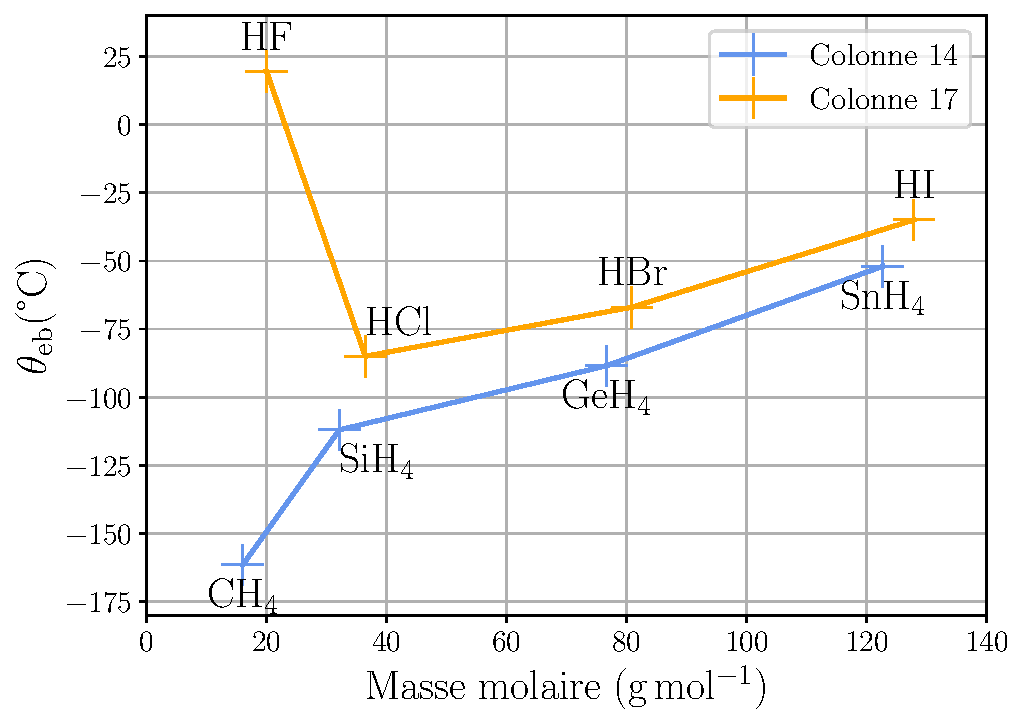
\includegraphics[width=\linewidth]{teb_hydro.pdf}
			\label{fig:tebhydro}
		\end{center}
	\end{minipage}
	\hfill
	\begin{minipage}[c]{.45\linewidth}
		\begin{center}
			\cfig{C(-[2,.7]H)(<:[5]H)(<[6]H)(-[7]H)}
		\end{center}
	\end{minipage}
}

\begin{blocQR}
	\item
	\QR{%
		En déduire le moment dipolaire de la molécule de méthane.
	}{%
		Par symétrie, la molécule de méthane ne possède pas de moment
		dipolaire permanent (les moments des quatre liaisons \ce{C-H} se
		compensent).
	}

	\QR{%
		En déduire la géométrie et le moment dipolaire des autres
		composés hydrogénés de la colonne 14.
	}{%
		Tous les éléments d'une même colonne ont le même nombre
		d'électrons de valence. Par conséquent, leurs composés
		hydrogénés ont tous la même structure, et en particulier leur
		géométrie est la même que celle de la molécule de méthane en ne
		changeant que l'atome central. De même, tous les composés
		hydrogénés de la colonne du carbone n'ont pas de moment
		dipolaire permanent.
	}
\end{blocQR}
\QR{%
	Pourquoi les composés hydrogénés des éléments de la colonne 14 ont-ils
	des température d'ébullition plus basses que celles des composés
	hydrogénés de la colonne 17~?
}{%
	Les éléments de la famille des halogènes sont bien plus
	électronégatifs que l'hydrogène et les molécules ne sont pas
	symétriques. Tous les composés de type \ce{H-X} où \ce{X} est un
	halogène sont donc polaires. Ainsi les forces de \textsc{Van der Waals}
	entre les composés hydrogénés de la colonne 17 sont plus importantes
	qu'entre les composés hydrogénés de la colonne 14. Ce qui explique les
	différences de température d'ébullition.
}

\QR{%
	Expliquer l'augmentation observée entre \ce{HCl} et \ce{HI}.
}{%
	La masse molaire de \ce{HI} est plus élevée que celle de \ce{HCl}, ce
	qui indique que la molécule est davantage polarisable. Les interactions
	de \textsc{Van der Waals} entre molécules sont donc plus fortes dans le
	cas de l'iode que dans le cas du chlore, ce qui explique la croissance
	observée.
}

\QR{%
	Proposer une explication à l'anomalie observée pour \ce{HF}.
}{%
	L'atome de fluor appartient à la deuxième période et il est fortement
	électronégatif. Des liaisons hydrogène peuvent donc se former entre
	molécules de \ce{HF}, ce qui n'est pas possible dans les autres espèces
	chimiques. Comme ces liaisons sont beaucoup plus fortes que les autres
	interactions faibles, elles expliquent la forte anomalie de température
	d'ébullition observée pour \ce{HF}.
}

\end{document}
